\subsection{ADC resampler} \label{subsec:ADCResampler}
The ADC resampler block is generating the 'acquire start' (trigger) inputs for the ADC control block. When 'acquire start' for the ADC control module is asserted, the ADC control will start a single conversion. The ADC resampler will generate $N$ amount of trigger pulses for the ADC control block, with $M$ frequency.

The amount of pulses generated, i.e. the sample size $N$, and the sample frequency $M$ along with a 'start' signal is set by a number registers in the internal memory that was described in section \refq{subsec:Memory}. The signals going into, or out of, the ADC resampler can be seen on figure \refq{fig:7_2_10_RESAMPLE_IO}.

\begin{figure}[H]
    \centering
    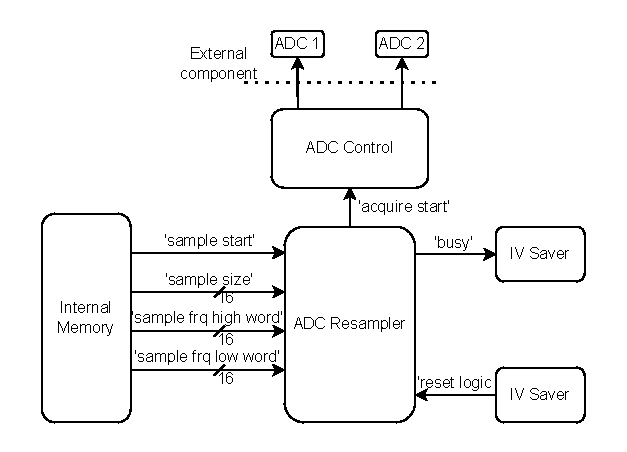
\includegraphics[clip, trim=0 0 0 0, width=0.9\textwidth]{Sections/7_SystemDesign/Figures/7_2_10_Resample_IO.pdf}
    \caption{A block diagram showing the I/O of the ADC resampler block. The ADC resampler also uses a \SIQ{200}{\mega\hertz} clock and a \SIQ{50}{\mega\hertz} clock, these are not shown on the block diagram.}
    \label{fig:7_2_10_RESAMPLE_IO}
\end{figure}

The module uses a Xilinx Direct Digital Synthesis (DDS) IP\cite{XILINXDDS} to generate the 'acquire start' pulses for the ADC control block. This is a black box component that was described briefly in section \refq{subsec:DAC_CONTROL} and it can be instantiated in an HDL project as a Vivado IP block for signal generation purposes. The output from the DDS module is a two's complement sine wave, but unlike the DAC control block, the ADC resampler block only requires the Numerically Controlled Oscillator portion of the DDS module in order to work, as it uses square waves and doesn't need to make use of the sine loop-up table in the DDS module. The ADC resampler block is getting a square wave from the DDS block by only using the MSb of the sine wave output. The DDS block uses a 48 bit control word, but only 32 bits are used as shown in the entity declaration in listing \refq{lst:7_2_10_ADCResampleEntity}.

\lstinputlisting[language=c ,style = c,firstnumber=1, linerange=37-49, caption={Code for DDS and DAC prescaler}, label={lst:7_2_10_ADCResampleEntity}]{Sections/7_SystemDesign/Code/adc_resampler.vhd}

The two signals, i\_sample\_frq\_low\_int\_mem\_reg and i\_sample\_frq\_high\_int\_mem\_reg, in lines 4 and 5 are concatenated with 0x0000 in order to form a 48 bit frequency control word for the DDS block. The DDS is using a \SIQ{50}{\mega\hertz} clock signal and this gives the DDS output a resolution of \SIQ{17.8}{\micro\hertz} as shown in equation \ref{eq:7_2_10_Fres}.

\begin{equation}\label{eq:7_2_10_Fres}
    f_{res} = \frac{f_{DDSCLK}}{2^N} = \frac{50e6}{2^{48}} = 1.776e-7
\end{equation}
This means the sample frequency of the ADC control block has a resolution of \SIQ{17.8}{\micro\hertz} as well.

The DDS block uses a phase accumulator and the size of the frequency control word affects the output jitter, a larger frequency control word reduces jitter as can be seen in the tests in appendix \refq{App:DDSJitter}. A 48 bit frequency control word is the largest that the DDS module can work with and is thus what is being used in this ADC resampler module.

The ADC resampler has been designed as the mealy machine shown in figure xyz




